\RequirePackage{fix-cm}
\documentclass[smallextended,envcountsame]{svjour3}
\smartqed
\usepackage{amsmath,amssymb}
\usepackage{stix}
\usepackage{graphicx,booktabs,array,float,xcolor}
\usepackage[colorlinks=true,linkcolor=blue,citecolor=blue,urlcolor=blue]{hyperref}
\setlength{\emergencystretch}{2.5em}
\setlength{\tabcolsep}{4pt}
\newfloat{algorithm}{tbp}{loa}
\floatname{algorithm}{Algorithm}
\newcommand{\todo}[1]{\textcolor{red}{\textbf{[TODO: #1]}}}
\newcommand{\step}[1]{\par\noindent\hangindent=1.5em\hangafter=1\textbf{Step #1.}\ }
\newcommand{\repo}{\url{https://github.com/mossaiby/iHaar}}
\journalname{Journal of Scientific Computing}

\begin{document}

\title{Real spectra and fast tensor solvers for midpoint quadratic-spline collocation on graded grids}
\titlerunning{Real spectra and fast tensor solvers for quadratic-spline collocation}

\author{Farshid Mossaiby}
\authorrunning{F. Mossaiby}

\institute{F. Mossaiby \at
  Department of Civil Engineering, University of Isfahan, Isfahan 81744-73441, Iran\\
  \email{mossaiby@eng.ui.ac.ir}}

\date{Received: date / Accepted: date}

\maketitle

\begin{abstract}
Fast diagonalization solves separable problems on tensor grids with a few dense matrix products, but it
requires one-dimensional operators that are diagonalizable with real eigenvalues. Collocation operators
on graded grids are not symmetric, so this property has to be proved. We prove it for midpoint
quadratic-spline collocation, which is the nodal form of the Haar wavelet collocation method (HWCM). An
exact three-term identity writes the second-derivative operator as $A^{-1}L$ with tridiagonal $A$ and $L$.
Using the theory of oscillation matrices, we show that this operator has real, simple and nonpositive
eigenvalues on every strictly increasing grid, for any combination of prescribed values and zero slopes
at the ends. Fast diagonalization is therefore well defined on arbitrary graded tensor grids. We
distinguish this algebraic guarantee from backward stability, which we observe on random and adversarial
grids, and from forward accuracy, which is limited by the conditioning of the discrete problem. On
uniform grids, a correction that keeps the eigenvectors raises the order to four for zero-flux
conditions. Applications include mass-conserving Allen--Cahn and Cahn--Hilliard schemes with a modified
energy law, resolving interfaces with about four nodes across the transition layer, and adaptive plane
elastostatics for compressible materials. In a benchmark against biquadratic finite elements on
identical grids, the method needed about one quarter of the unknowns.
\keywords{Spline collocation \and Haar wavelet collocation \and Fast diagonalization \and Oscillation matrices \and Phase-field models \and Adaptive refinement}
\subclass{65N35 \and 65F15 \and 15B48 \and 65N22 \and 65M70 \and 74S25}
\end{abstract}

%==========================================================================
\section{Introduction}\label{sec:intro}
%==========================================================================
The Haar wavelet collocation method (HWCM)~\cite{chen1997haar,lepik2005numerical,lepik2011solving,lepik2014book}
is widely used in applied mechanics for beams, plates, shells and functionally graded
structures~\cite{majak2015accuracy,majak2015convergence,majak2018higher}. The highest derivative of the
unknown is expanded in Haar functions, the lower derivatives follow by exact integration, and the
equation is enforced at cell midpoints. Higher-order variants~\cite{majak2018higher,ratas2021solving} and
graded grids based on non-uniform Haar functions~\cite{dubeau2004nonuniform,lepik2008nonuniform,oruc2019nonuniform}
are available. In two dimensions, however, all equations are usually assembled into one dense matrix of
size $N^2\times N^2$, which becomes impractical beyond about $64\times64$ cells.

In terms of nodal values, HWCM is midpoint quadratic-spline collocation
(QSC)~\cite{houstis1988quadratic,christara1994quadratic,christara2006optimal}, and it uses the same
functions as quadratic isogeometric collocation~\cite{auricchio2010isogeometric,schillinger2013isogeometric}.
On tensor grids, separable problems can be solved by fast diagonalization~\cite{lynch1964direct}, which
reduces two- and three-dimensional problems to dense matrix products and fast transforms. It requires
each one-dimensional operator to be diagonalizable with real eigenvalues. For symmetric finite-element
and isogeometric Galerkin operators this is automatic~\cite{sangalli2016isogeometric}. Collocation
operators are generally not symmetric, and for them the property has to be proved. For Hermite-cubic
orthogonal spline collocation at Gauss points it is known~\cite{dyksen1987tensor,sun1999spectral}, and it
underlies the matrix decomposition algorithms of Bialecki and Fairweather~\cite{bialecki1995matrix,bialecki2011matrix}.
For QSC, fast solvers exist on uniform grids~\cite{christara2002fast}. To our knowledge, a spectral
guarantee has not been established for midpoint QSC on arbitrary non-uniform partitions. There, the
collocation operator is not symmetric and is not symmetrized by quadrature weights, so a different
argument is needed.

The main result of this paper (Theorem~\ref{thm:spectrum}) provides this guarantee. On every strictly
increasing grid, and for every combination of prescribed values and zero slopes at the ends, the
second-derivative operator has real, simple and nonpositive eigenvalues. The proof combines an exact
three-term identity (Theorem~\ref{thm:identity}) with the theory of oscillation
matrices~\cite{gantmacher2002oscillation,fallat2011totally}, and it is given in full in
Appendix~\ref{app:proofs}. We then examine what the result does and does not provide in floating-point
arithmetic, distinguishing well-definedness, backward stability and forward accuracy
(Section~\ref{sec:robust}). We also demonstrate its consequences in three settings: verification problems on
uniform and graded grids, Allen--Cahn and Cahn--Hilliard computations with thin interfaces, and
elastostatics with traction boundaries and adaptive refinement at corner singularities.
Table~\ref{tab:closest} compares the method with the closest existing approaches. Secondary proofs and
additional tables are collected in the Supplementary Material, and the code is available at \repo.

\begin{table}[t]\centering\footnotesize
\caption{Comparison with the closest spline-collocation approaches, to the best of our knowledge.
``Spectrum'' refers to the one-dimensional collocation operator used by fast diagonalization or matrix
decomposition.}\label{tab:closest}
\begin{tabular}{p{0.14\textwidth}p{0.18\textwidth}p{0.13\textwidth}p{0.235\textwidth}p{0.175\textwidth}}
\toprule
Method & Trial space and collocation points & Grids & Spectrum & Fast solver\\
\midrule
Classical HWCM~\cite{lepik2011solving,oruc2019nonuniform} & integrated Haar ($C^1$ quadratics); midpoints & uniform or a~priori graded & not analysed & none (dense $N^2\times N^2$ solve)\\
Hermite-cubic OSC~\cite{dyksen1987tensor,sun1999spectral,bialecki1995matrix} & $C^1$ cubics; two Gauss points per cell & partitions as in the cited works & real, distinct eigenvalues established & matrix decomposition; FFT on uniform grids\\
QSC~\cite{houstis1988quadratic,christara2002fast,christara2006optimal} & $C^1$ quadratics; midpoints (optimal variants perturbed) & uniform; non-uniform analysed for convergence & symmetric, trigonometric eigenvectors on uniform grids & FFT and matrix decomposition on uniform grids\\
Quadratic IGA collocation~\cite{auricchio2010isogeometric,schillinger2013isogeometric,delorenzis2015isogeometric} & B-splines; Greville or superconvergent points & arbitrary knots; local refinement & not established for collocation; Galerkin pencils symmetric~\cite{sangalli2016isogeometric} & direct or Krylov\\
This work & $C^1$ quadratics; midpoints & arbitrary graded tensor grids & real, simple, nonpositive on every grid (Theorem~\ref{thm:spectrum}) & fast diagonalization on any tensor grid; DCT/DST on uniform grids\\
\bottomrule
\end{tabular}
\end{table}

%==========================================================================
\section{Midpoint quadratic-spline collocation}\label{sec:method}
%==========================================================================
\subsection{Nodal form of Haar wavelet collocation}
Let $a=t_0<t_1<\dots<t_N=b$, with $N\ge2$, be the grid, with cells $I_k=[t_{k-1},t_k]$ of width $h_k$,
midpoints $m_k$, and midpoint spacings $d_k=(h_k+h_{k+1})/2$. HWCM expands $u''$ in Haar functions and
integrates twice. On a given grid, the Haar functions span exactly the functions that are constant on each
cell, so the Haar coefficients carry the same information as the cell values $c_k=u''|_{I_k}$.
Integrating twice gives piecewise quadratics with continuous slopes, that is, $C^1$ quadratic splines.
We use the values $U_k=u(m_k)$ at the cell midpoints, which are the HWCM collocation values, as unknowns.

\begin{theorem}[Three-term identity]\label{thm:identity}
Let $s$ be a $C^1$ quadratic spline on the grid, with $U_k=s(m_k)$ and $c_k=s''|_{I_k}$. For $2\le k\le N-1$,
\begin{equation}\label{eq:interior}
\frac{U_{k+1}-U_k}{d_k}-\frac{U_k-U_{k-1}}{d_{k-1}}
=\frac{h_{k-1}^2}{8d_{k-1}}c_{k-1}+\Big(h_k-\frac{h_k^2}{8d_{k-1}}-\frac{h_k^2}{8d_k}\Big)c_k+\frac{h_{k+1}^2}{8d_k}c_{k+1}.
\end{equation}
At the left end, with $g_0=s(a)$,
\begin{align}
\frac{U_2-U_1}{d_1}-\frac{2(U_1-g_0)}{h_1}&=\Big(\frac{3h_1}{4}-\frac{h_1^2}{8d_1}\Big)c_1+\frac{h_2^2}{8d_1}c_2 &&\text{(value prescribed)},\label{eq:dirrow}\\
\frac{U_2-U_1}{d_1}&=\Big(h_1-\frac{h_1^2}{8d_1}\Big)c_1+\frac{h_2^2}{8d_1}c_2 &&\text{(if } s'(a)=0),\label{eq:neurow}
\end{align}
and symmetrically at the right end. In matrix form, $LU+b=Ac$, where $L$ is a tridiagonal difference
matrix, $A$ a tridiagonal averaging matrix, and $b$ contains the prescribed end values.
\end{theorem}

\begin{corollary}[Invertibility and solvability]\label{cor:ops}
For every grid and every combination of end conditions, $A$ has a positive diagonal and positive
off-diagonal entries, and it is strictly diagonally dominant by columns, hence invertible. With zero-slope ends, the columns of $A$
sum to the cell widths $h_k$. The collocation problem $s''(m_k)=f(m_k)$, $k=1,\dots,N$, has a
unique solution if a value is prescribed at one or both ends. If the slope vanishes at both ends, the
constants form the kernel of $L$, and a solution exists if and only if $\sum_kh_kf(m_k)=0$; it is then
unique up to an additive constant, which can be fixed, for example, by prescribing $\sum_kh_kU_k$.
\end{corollary}

The second derivative at the nodes is therefore $c=D_2U+e$, where $D_2=A^{-1}L$ and the vector $e$ collects the boundary terms.
Instead of the dense integration matrices of classical HWCM, only two tridiagonal matrices need to be
assembled. Slopes follow in closed form as well, which gives the first-derivative matrix $D_1$ and the
end slopes needed for traction conditions (Algorithm~1). Proofs of Theorem~\ref{thm:identity} and
Corollary~\ref{cor:ops} are given in Appendix~\ref{app:proofs}.

\begin{algorithm}[t]\small\hrule\smallskip
\noindent\textbf{Algorithm 1: one-dimensional operators} (\texttt{ihaar/core.py}, class \texttt{Grid1D}).
Input: knots $t_0<\dots<t_N$ and the type of each end (value prescribed, or zero slope).
\step{1} Compute $h_k$, $m_k$ and $d_k$, and assemble the tridiagonal matrices $L$ and $A$ from~\eqref{eq:interior}--\eqref{eq:neurow}.
\step{2} Factorize $A$ (tridiagonal LU) and form $D_2=A^{-1}L$ and the boundary vectors $e_i=A^{-1}b_i$.
\step{3} Form the first-derivative matrix $D_1=\mathbf 1r^{\mathsf T}+TD_2$, where $T_{kj}=h_j$ for $j<k$, $T_{kk}=h_k/2$, and $r$ encodes the end slope $\sigma_0=2(U_1-g_0)/h_1-c_1h_1/4$.
\step{4} Form the end slopes $s'(a)=\sigma_0$ and $s'(b)=\sigma_0+\sum_kh_kc_k$ as row vectors, for traction conditions.
\smallskip\hrule
\end{algorithm}

\subsection{Main result: a real, simple and nonpositive spectrum on every grid}
\begin{theorem}[Spectrum on every grid]\label{thm:spectrum}
Let $a=t_0<t_1<\dots<t_N=b$, with $N\ge2$, be any strictly increasing knot vector, and let either the
value or a zero slope be prescribed at each end. Then $D_2=A^{-1}L$ has $N$ real and simple eigenvalues,
and it is diagonalizable with a real eigenvector matrix $V$. If a value is prescribed at one or both ends,
all eigenvalues are negative. If the slope vanishes at both ends, exactly one eigenvalue is zero, with the
constant vector as eigenvector, and all others are negative.
\end{theorem}

The proof (Appendix~\ref{app:proofs}) uses only three properties of the identity: $A$ is a positive,
column-diagonally-dominant tridiagonal matrix, $-L$ is a tridiagonal M-matrix, and the columns of $A$ sum
to the cell widths. These properties make $A$ and $(-L)^{-1}$ totally nonnegative, and their product
oscillatory in the sense of Gantmacher and Krein~\cite{gantmacher2002oscillation}, whose eigenvalues are
real, positive and simple. No assumption on the grading, such as a bounded ratio between neighbouring
cells, is needed. The result extends immediately to tensor-product operators.

\begin{corollary}[Tensor-product operators]\label{cor:tensor}
On a tensor grid in $d$ dimensions, with end conditions as in Theorem~\ref{thm:spectrum} in each direction,
every operator $\sum_m\alpha_mD_2^{(m)}+\gamma I$, with $\alpha_m>0$ and $D_2^{(m)}$ acting along direction
$m$, is diagonalized by $V_1\otimes\dots\otimes V_d$, with the real eigenvalues
$\sum_m\alpha_m\lambda^{(m)}_{i_m}+\gamma$. It is nonsingular whenever $\gamma<0$, or $\gamma=0$ and a value
is prescribed at some end in at least one direction.
\end{corollary}

Theorem~\ref{thm:spectrum} is an algebraic statement: fast diagonalization is well defined on any grid,
without complex arithmetic or defective matrices. It does not bound the conditioning $\kappa(V)$ of the
eigenvector matrix, and it says nothing about the conditioning of the discrete problem itself. These
floating-point questions are examined in Section~\ref{sec:robust}.

\subsection{Uniform grids: cosine transforms, fourth order and mass conservation}
\begin{proposition}[Uniform grids]\label{thm:fourth}
On a uniform grid, $D_2=\frac{8}{h^2}\delta^2(8I+\delta^2)^{-1}$, where $\delta^2$ is the three-point second
difference with end entries $-3$ (prescribed value) or $-1$ (zero slope). It is symmetric and diagonalized
by the discrete sine (prescribed values) or cosine (zero slope) transform, with eigenvalues in
$[-8/h^2,0]$. The corrected operator
\begin{equation}\label{eq:D24}
D_2^{(4)}=D_2+\tfrac{h^2}{24}D_2^2
\end{equation}
has the same eigenvectors, is negative semidefinite, and is fourth-order accurate for smooth solutions
of zero-flux or periodic problems whose odd normal derivatives vanish at the ends. For general prescribed
values, the order remains two.
\end{proposition}

\begin{proposition}[Exact mass conservation]\label{prop:mass}
With zero slope at both ends, $h^{\mathsf T}D_2=0$ on any grid, where $h=(h_k)$, so the weighted sum
$\sum_kh_kU_k$ is conserved by evolutions of the form $\dot U=D_2W$. On a uniform grid, this sum equals the
exact integral of the spline.
\end{proposition}

Plain HWCM has half the error constant of the three-point difference ($-h^2/24$ against $h^2/12$), so it is
about twice as accurate on the same grid. The fourth-order correction costs nothing, because in the
transform domain it only changes the eigenvalues. Proofs of Propositions~\ref{thm:fourth}
and~\ref{prop:mass} are given in the Supplementary Material.

%==========================================================================
\section{Fast solvers in two and three dimensions}\label{sec:tensor}
%==========================================================================
On a rectangle, the unknowns form a matrix $U_{ij}$, and the one-dimensional operators act along the grid
lines: $U_{xx}=D_2^xU$ and $U_{yy}=U(D_2^y)^{\mathsf T}$, plus boundary terms. An equation such as
$\alpha u_{xx}+\beta u_{yy}+\gamma u=f$ becomes a Sylvester matrix equation. With the eigendecompositions
$D_2^x=V_x\Lambda_xV_x^{-1}$ and $D_2^y=V_y\Lambda_yV_y^{-1}$, which exist by Theorem~\ref{thm:spectrum},
its solution is
\begin{equation}\label{eq:fdm}
U=V_x\Big[\big(V_x^{-1}\tilde FV_y^{-\mathsf T}\big)\oslash\big(\alpha\lambda^x_i+\beta\lambda^y_j+\gamma\big)_{ij}\Big]V_y^{\mathsf T},
\end{equation}
where $\oslash$ denotes entrywise division. This takes four dense matrix products after a one-time
eigendecomposition. In three dimensions the cost is $O(N^4)$, and on uniform grids fast cosine
transforms reduce it to $O(N^d\log N)$. All operations are dense matrix products, fast transforms or
pointwise operations. The code takes the array library (NumPy or CuPy) as a parameter, so the same code
runs on CPUs and GPUs.

%==========================================================================
\section{Phase-field solvers}\label{sec:pf}
%==========================================================================
We solve the Allen--Cahn (AC) and Cahn--Hilliard (CH) equations with zero-flux boundaries,
$u_t=-\mathcal G\mu$, $\mu=-\varepsilon^2\Delta u+u^3-u$, with $\mathcal G=I$ for AC and $\mathcal G=-\Delta$
for CH. The parameter $\varepsilon$ sets the interface thickness. Across an equilibrium interface
$u\approx\tanh(d/\sqrt2\varepsilon)$, where $d$ is the distance to the interface. With $K$ the discrete
$-\Delta$, $\bar u=2u^n-u^{n-1}$, and a scalar auxiliary variable $r$~\cite{shen2018scalar}, the
stabilized SAV-BDF2 scheme reads
\begin{align}
\frac{3u^{n+1}-4u^n+u^{n-1}}{2\Delta t}&=-G\mu^{n+1},\label{eq:sav1}\\
\mu^{n+1}&=\varepsilon^2Ku^{n+1}+S(u^{n+1}-\bar u)+r^{n+1}\bar b,\label{eq:sav1b}\\
3r^{n+1}-4r^n+r^{n-1}&=\tfrac12\langle\bar b,3u^{n+1}-4u^n+u^{n-1}\rangle_h,\label{eq:sav2}
\end{align}
where $\bar b=f(\bar u)/\sqrt{E_1(\bar u)+C}$ is the scaled nonlinearity and $S\ge0$ a stabilization
constant. Each step costs one forward and one inverse transform (Algorithm~2). The scheme works in three dimensions
as well; a three-dimensional accuracy test is reported in Table~S18.

\begin{theorem}[Mass and modified energy]\label{thm:energy}
On a uniform grid, for every time step and every $S\ge0$, the scheme has a unique solution, the CH scheme
conserves the discrete mass exactly, and a modified energy never increases. The proof is given in the
Supplementary Material.
\end{theorem}

It is important to know what this guarantee does not cover. It concerns a \emph{modified} energy. That
the physical energy decreases, that $u$ stays bounded, and that interfaces move correctly are separate
properties, which we only observe in our tests. For thin interfaces they need stabilization: with
$S=0$, a computation with $\varepsilon=0.0015$ produced values of $|u|$ around 30 to 70 while the
modified energy kept decreasing, whereas $S=4$ kept $|u|\le1.04$ (Table~\ref{tab:savstab}). A systematic study (Table~S17) shows that the smallest $S$ that keeps the ratio $\xi=r/\sqrt{E_1+C}$
close to one is the most accurate: $S\approx1$ to 2 for time steps up to $\varepsilon^2$, and 2 to 4 for
larger steps. Even then, steps much larger than $\varepsilon^2$ give wrong interface motion, so $\xi\approx1$
does not replace checking the time step. These are empirical recommendations, not proved thresholds.

\begin{algorithm}[t]\small\hrule\smallskip
\noindent\textbf{Algorithm 2: one SAV-BDF2 time step} (\texttt{ihaar/phasefield.py}).
Precomputed: the transform $\mathcal T$ (DCT-II, or the eigenvectors $V$), the symbols $\hat\lambda$ of
$-K$, $\hat G=1$ (AC) or $\hat\lambda$ (CH), and $\hat S_2=3+2\Delta t\,\hat G(\varepsilon^2\hat\lambda+S)$.
Stored from previous steps: $\hat u^n$, $\hat u^{n-1}$, $u^n$, $u^{n-1}$, $r^n$, $r^{n-1}$.
\step{1} Compute $\bar u=2u^n-u^{n-1}$ and $\bar b=f(\bar u)/\sqrt{E_{1,h}(\bar u)+C}$, and transform, $\hat{\bar b}=\mathcal T\bar b$ (one forward transform).
\step{2} Compute $\hat g=4\hat u^n-\hat u^{n-1}$, $\hat p=(\hat g+2\Delta t\,S\hat G\,\hat{\bar u})/\hat S_2$ and $\hat q=-2\Delta t\,\hat G\hat{\bar b}/\hat S_2$.
\step{3} Update the scalar, $r^{n+1}=\big(4r^n-r^{n-1}+\tfrac12\langle\hat{\bar b},3\hat p-\hat g\rangle\big)/\big(3-\tfrac32\langle\hat{\bar b},\hat q\rangle\big)$, with inner products evaluated in the orthonormal transform domain.
\step{4} Set $\hat u^{n+1}=\hat p+r^{n+1}\hat q$ and $u^{n+1}=\mathcal T^{-1}\hat u^{n+1}$ (one inverse transform).
\smallskip\hrule
\end{algorithm}

%==========================================================================
\section{Elastostatics}\label{sec:elast}
%==========================================================================
For plane strain we enforce the Navier equations at the cell midpoints. Because $u$ and $v$ are coupled,
we use GMRES, preconditioned by two decoupled fast-diagonalization solves per iteration, one for each
displacement component. For compressible materials the number of iterations does not grow with the grid;
as Poisson's ratio approaches one half it grows strongly (Tables~S1 and~S2), so the solver is intended for
compressible materials. On a traction edge, the edge displacements become unknowns, and
$\boldsymbol\sigma\mathbf n=\mathbf t$ is enforced at the edge midpoints. The normal derivatives come from
the end slopes of Algorithm~1, and the tangential derivatives from $D_1$ along the edge. Where two traction
edges meet, the two normal stresses are prescribed. Unlike quadratic isogeometric collocation, where
pointwise traction conditions can lose accuracy and an ``enhanced'' boundary equation is
recommended~\cite{delorenzis2015isogeometric}, plain collocation stays second-order accurate here. With tractions on two adjacent edges and $\nu=0.3$,
the relative $H^1$ error decreases from $4.3\times10^{-3}$ at $N=16$ to $1.7\times10^{-5}$ at
$N=256$ (observed rate 2.00), and the largest displacement error on the traction edges is
$1.8\times10^{-5}$; on a geometric grid graded toward the traction edge with cell-size ratio up to
85, the rate is again two (Tables~S9 and~S10). In the preconditioner, a traction edge is treated as a zero-slope end,
which is again covered by Theorem~\ref{thm:spectrum}.

For adaptivity we use the Haar coefficients directly. The finest-level Haar coefficient of $u''$ is
proportional to the jump of $u''$ between neighbouring cells, and this jump measures the local error of
the gradient. For each cell of the $x$-direction grid we compute
\begin{equation}\label{eq:indicator}
\eta^x_i{}^2=h^x_i{}^3\sum_jh^y_j\,\tfrac12\Big([\![u_{xx}]\!]_{i-\frac12,j}^2+[\![u_{xx}]\!]_{i+\frac12,j}^2\Big),
\end{equation}
summed over both displacement components, and similarly in $y$. Algorithm~3 marks and bisects the cells
with the largest indicators. The indicator is heuristic, in the sense that no error bound is proved for it,
but in all our tests it followed the true error closely.

\begin{algorithm}[t]\small\hrule\smallskip
\noindent\textbf{Algorithm 3: adaptive elastostatics} (\texttt{ihaar/elasticity\_bc.py}).
\step{1} Start from a uniform tensor grid, for example $8\times8$ cells.
\step{2} Build the one-dimensional operators (Algorithm~1) and the preconditioner factorizations, and solve with right-preconditioned GMRES (relative tolerance $10^{-10}$, restart length 60 to 80).
\step{3} Compute the indicators $\eta^x_i$ and $\eta^y_j$ from~\eqref{eq:indicator}.
\step{4} Mark the smallest set of one-dimensional cells, in both directions together, that carries a fraction $\theta=0.6$ of $\sum\eta^2$ (D\"orfler marking~\cite{dorfler1996convergent}), and bisect them.
\step{5} Bisect further until neighbouring cells differ in size by at most a factor of two, and return to Step~2.
\smallskip\hrule
\end{algorithm}

%==========================================================================
\section{Results}\label{sec:results}
%==========================================================================
All computations ran in double precision on the system described in Table~\ref{tab:env}; absolute
timings depend on this hardware and software. Every number is produced by the scripts of the repository,
and the tables are generated from the stored results.

\begin{table}[t]\centering\footnotesize
\caption{Computing environment and timing protocol.}\label{tab:env}
\begin{tabular}{p{0.22\textwidth}p{0.70\textwidth}}
\toprule
item & value\\
\midrule
CPU & AMD Ryzen 7 5800U (8 cores, 16 threads, 1.90 GHz base clock)\\
operating system & Windows 10\\
software & Python 3.11.9, NumPy 2.4.6, SciPy 1.17.1\\
BLAS/LAPACK & scipy-openblas 0.3.31.188.0\\
threads & 16 logical CPUs; BLAS threading: default\\
memory & 16 GB\\
GPU (Table~\ref{tab:perf}) & NVIDIA GeForce RTX 3050 Ti Laptop GPU (4 GB)\\
timing protocol & wall-clock time (\texttt{time.perf\_counter}); solve times are medians of 3 to 5 repetitions; setup and assembly are reported separately and are not amortized\\
\bottomrule
\end{tabular}
\end{table}

\subsection{Verification}\label{sec:verify}
Table~\ref{tab:poisson} reports the maximum nodal error for $-\Delta u=f$ with prescribed values and
$u=e^x\sin\pi y+x^2y$, on uniform and on Chebyshev-graded grids, and for $(I-\Delta)u=f$ with zero-slope
conditions and $u=\cos\pi x\cos2\pi y+0.3\cos3\pi x$. The plain operator converges at second order on both
grid families, and the corrected operator at fourth order when its conditions hold. Second-order
convergence was also observed for smooth elastostatic solutions with prescribed displacements and with
tractions, in three dimensions on uniform and graded grids, and for the Cahn--Hilliard equation, where the
corrected operator gives fourth order (Tables~S8, S9, S18 and~S13).

\begin{table}[t]\centering\footnotesize
\caption{Maximum nodal error and observed convergence rates for two model problems.}\label{tab:poisson}
\textit{(a) Prescribed values, $-\Delta u=f$, operator $D_2$}\\[2pt]
\begin{tabular}{r cc cc}
\toprule
& \multicolumn{2}{c}{uniform grid} & \multicolumn{2}{c}{Chebyshev-graded grid}\\
$N$ & error & rate & error & rate\\
\midrule
8 & $6.50{\times}10^{-3}$ & -- & $3.96{\times}10^{-3}$ & --\\
16 & $1.66{\times}10^{-3}$ & 1.97 & $1.15{\times}10^{-3}$ & 1.79\\
32 & $4.18{\times}10^{-4}$ & 1.99 & $2.96{\times}10^{-4}$ & 1.95\\
64 & $1.05{\times}10^{-4}$ & 2.00 & $7.46{\times}10^{-5}$ & 1.99\\
128 & $2.61{\times}10^{-5}$ & 2.00 & $1.87{\times}10^{-5}$ & 2.00\\
256 & $6.54{\times}10^{-6}$ & 2.00 & $4.67{\times}10^{-6}$ & 2.00\\
512 & $1.63{\times}10^{-6}$ & 2.00 & $1.17{\times}10^{-6}$ & 2.00\\
\bottomrule
\end{tabular}

\medskip
\textit{(b) Zero-slope conditions, $(I-\Delta)u=f$, uniform grid}\\[2pt]
\begin{tabular}{r cc cc}
\toprule
& \multicolumn{2}{c}{$D_2$} & \multicolumn{2}{c}{$D_2^{(4)}$}\\
$N$ & error & rate & error & rate\\
\midrule
8 & $3.05{\times}10^{-2}$ & -- & $4.69{\times}10^{-3}$ & --\\
16 & $9.11{\times}10^{-3}$ & 1.74 & $3.15{\times}10^{-4}$ & 3.89\\
32 & $2.38{\times}10^{-3}$ & 1.94 & $2.01{\times}10^{-5}$ & 3.98\\
64 & $6.01{\times}10^{-4}$ & 1.98 & $1.26{\times}10^{-6}$ & 3.99\\
128 & $1.51{\times}10^{-4}$ & 2.00 & $7.87{\times}10^{-8}$ & 4.00\\
256 & $3.77{\times}10^{-5}$ & 2.00 & $4.92{\times}10^{-9}$ & 4.00\\
512 & $9.42{\times}10^{-6}$ & 2.00 & $3.08{\times}10^{-10}$ & 4.00\\
\bottomrule
\end{tabular}
\end{table}

\subsection{Well-definedness, backward stability and forward accuracy}\label{sec:robust}
Three different properties must be distinguished. Theorem~\ref{thm:spectrum} guarantees that fast
diagonalization is \emph{well defined} on every grid. Whether it is \emph{backward stable}, that is, whether
the computed solution exactly solves a slightly perturbed problem, depends on the conditioning $\kappa(V)$ of
the eigenvectors, which the theorem does not bound. Whether the computed solution is \emph{accurate} in the
forward sense depends, in addition, on the conditioning of the discrete problem itself. For the Sylvester
operator $U\mapsto\alpha D_2^xU+\beta U(D_2^y)^{\mathsf T}+\gamma U$ we use the estimate
$\kappa_{\mathrm{Syl}}=\kappa(V_x)\kappa(V_y)\max|\mu_{ij}|/\min|\mu_{ij}|$, where $\mu_{ij}$ are its
eigenvalues; it bounds the normwise sensitivity and may be pessimistic.

We tested backward stability against the Bartels--Stewart algorithm~\cite{bartels1972solution} on 8760 random
graded grids (Table~S4) and on adversarial families: alternating cell sizes, isolated tiny end cells,
clusters of small cells, unbounded random sizes, and geometric grading up to $10^{12}$
(Table~\ref{tab:fdmstab}; random grids in Table~S15). The eigenvalues were real in every case, $\kappa(V)$
stayed below 85, and the backward error of fast diagonalization stayed at round-off level, between
$10^{-30}$ and $6\times10^{-15}$. Forward accuracy is a different matter. On the most extreme grids, the
solutions of the two backward-stable methods differ by up to $2\times10^{10}$ in relative terms, and every
such case has $\kappa_{\mathrm{Syl}}\gtrsim10^{16}$, beyond the reciprocal of the machine precision. These
problems are intrinsically ill conditioned: their eigenvalues span many orders of magnitude because the cell
sizes do, and no solver can compute them accurately in double precision.

The implementation therefore uses two safeguards with different purposes. The first concerns backward
stability: after each solve it evaluates the normwise backward error, at the cost of two matrix products,
and repeats the solve with Bartels--Stewart if $\kappa(V)>10^6$ or the backward error exceeds $10^{-12}$.
This never triggered in our computations, and the fallback costs 42 to 62 times more on our hardware (Table~S19). The second
concerns forward accuracy: the code computes $\kappa_{\mathrm{Syl}}$ and flags the problem as sensitive when
$\kappa_{\mathrm{Syl}}$ times the machine precision exceeds $10^{-6}$. This flag is a warning, not a remedy,
since neither solver can improve the accuracy of an ill-conditioned problem. On all grids generated by the
refinement algorithm, whose neighbour ratio is at most two, $\kappa(V)$ stayed below 25.

Table~\ref{tab:cost} shows the practical gain over classical HWCM. On our hardware, the dense HWCM solve takes
0.7~s at $64\times64$ cells and is infeasible beyond that, whereas the cosine-transform solver handles
$10^6$ unknowns in 0.04~s.

\begin{table}[t]\centering\footnotesize
\caption{Adversarial grid families ($N=256$): eigenvector conditioning $\kappa(V)$, condition estimate
$\kappa_{\mathrm{Syl}}$ of the Sylvester problem, normwise backward errors of fast diagonalization (FDM) and
Bartels--Stewart (B--S), and relative difference of the two solutions.}\label{tab:fdmstab}
\textit{(a) Grid, eigenvector conditioning and condition estimate of the Sylvester problem}\\[2pt]
\begin{tabular}{p{0.30\textwidth}c c c c}
\toprule
grid family ($N=256$) & ends & $h_{\max}/h_{\min}$ & $\kappa(V)$ & $\kappa_{\mathrm{Syl}}$\\
\midrule
alternating, ratio 10 & values & $1{\times}10^{1}$ & 2 & $3{\times}10^{6}$\\
alternating, ratio 10 & slope & $1{\times}10^{1}$ & 2 & $2{\times}10^{7}$\\
alternating, ratio 100 & values & $1{\times}10^{2}$ & 2 & $3{\times}10^{8}$\\
alternating, ratio 100 & slope & $1{\times}10^{2}$ & 3 & $2{\times}10^{8}$\\
alternating, ratio 1000 & values & $1{\times}10^{3}$ & 2 & $3{\times}10^{10}$\\
alternating, ratio 1000 & slope & $1{\times}10^{3}$ & 3 & $2{\times}10^{9}$\\
end cells $10^{-6}$ & values & $1{\times}10^{6}$ & 1 & $2{\times}10^{16}$\\
end cells $10^{-6}$ & slope & $1{\times}10^{6}$ & 3 & $3{\times}10^{12}$\\
geometric, $10^6$ & values & $1{\times}10^{6}$ & 9 & $2{\times}10^{16}$\\
geometric, $10^6$ & slope & $1{\times}10^{6}$ & 47 & $9{\times}10^{18}$\\
geometric, $10^{12}$ & values & $1{\times}10^{12}$ & 6 & $3{\times}10^{27}$\\
geometric, $10^{12}$ & slope & $1{\times}10^{12}$ & 83 & $6{\times}10^{30}$\\
random, unbounded & values & $9{\times}10^{5}$ & 13 & $2{\times}10^{16}$\\
random, unbounded & slope & $9{\times}10^{5}$ & 15 & $2{\times}10^{16}$\\
cluster of $10^{-4}$ cells & values & $1{\times}10^{4}$ & 40 & $5{\times}10^{15}$\\
cluster of $10^{-4}$ cells & slope & $1{\times}10^{4}$ & 40 & $9{\times}10^{16}$\\
\bottomrule
\end{tabular}

\medskip
\textit{(b) Normwise backward errors and relative difference of the two solutions}\\[2pt]
\begin{tabular}{p{0.30\textwidth}c ccc}
\toprule
grid family ($N=256$) & ends & FDM & B--S & difference\\
\midrule
alternating, ratio 10 & values & $4{\times}10^{-16}$ & $6{\times}10^{-16}$ & $2{\times}10^{-12}$\\
alternating, ratio 10 & slope & $1{\times}10^{-15}$ & $2{\times}10^{-15}$ & $3{\times}10^{-10}$\\
alternating, ratio 100 & values & $5{\times}10^{-17}$ & $6{\times}10^{-17}$ & $3{\times}10^{-11}$\\
alternating, ratio 100 & slope & $1{\times}10^{-15}$ & $2{\times}10^{-15}$ & $3{\times}10^{-10}$\\
alternating, ratio 1000 & values & $1{\times}10^{-17}$ & $6{\times}10^{-18}$ & $3{\times}10^{-10}$\\
alternating, ratio 1000 & slope & $4{\times}10^{-15}$ & $2{\times}10^{-15}$ & $4{\times}10^{-9}$\\
end cells $10^{-6}$ & values & $6{\times}10^{-16}$ & $2{\times}10^{-17}$ & $4{\times}10^{-1}$\\
end cells $10^{-6}$ & slope & $7{\times}10^{-15}$ & $1{\times}10^{-16}$ & $6{\times}10^{-7}$\\
geometric, $10^6$ & values & $5{\times}10^{-22}$ & $3{\times}10^{-22}$ & $3{\times}10^{-13}$\\
geometric, $10^6$ & slope & $5{\times}10^{-17}$ & $5{\times}10^{-17}$ & $1{\times}10^{-7}$\\
geometric, $10^{12}$ & values & $6{\times}10^{-28}$ & $1{\times}10^{-16}$ & $6{\times}10^{7}$\\
geometric, $10^{12}$ & slope & $4{\times}10^{-17}$ & $1{\times}10^{-16}$ & $2{\times}10^{10}$\\
random, unbounded & values & $1{\times}10^{-15}$ & $7{\times}10^{-17}$ & $2{\times}10^{-5}$\\
random, unbounded & slope & $4{\times}10^{-15}$ & $2{\times}10^{-16}$ & $9{\times}10^{-4}$\\
cluster of $10^{-4}$ cells & values & $5{\times}10^{-16}$ & $1{\times}10^{-16}$ & $2{\times}10^{-6}$\\
cluster of $10^{-4}$ cells & slope & $4{\times}10^{-16}$ & $1{\times}10^{-16}$ & $2{\times}10^{-4}$\\
\bottomrule
\end{tabular}
\end{table}
\begin{table}[t]\centering\footnotesize
\caption{Wall time in seconds of one solve with $N^2$ unknowns, on the CPU of Table~\ref{tab:env}. ``Dense'' is the classical
HWCM approach.}\label{tab:cost}
\begin{tabular}{rr ccccc}
\toprule
$N$ & unknowns & dense & B--S & FDM setup & FDM & DCT\\
\midrule
16 & 256 & 0.005 & 0.000 & 0.001 & 0.000 & 0.000\\
32 & 1024 & 0.034 & 0.000 & 0.000 & 0.000 & 0.000\\
64 & 4096 & 0.732 & 0.002 & 0.002 & 0.000 & 0.000\\
128 & 16384 & -- & 0.034 & 0.006 & 0.000 & 0.000\\
256 & 65536 & -- & 0.128 & 0.021 & 0.001 & 0.001\\
512 & 262144 & -- & 1.317 & 0.093 & 0.006 & 0.005\\
1024 & 1048576 & -- & 8.369 & 0.466 & 0.055 & 0.037\\
\bottomrule
\end{tabular}
\end{table}

\subsection{Elastostatics: a crack-like corner and a comparison with finite elements}\label{sec:q2}
We use the exact Mode-I field of a re-entrant corner of opening $3\pi/2$~\cite{williams1952stress}, whose
displacements behave like $r^{0.544}$ near the corner. The square is placed so that its top edge lies on a
traction-free face and the singular point is at the end of that face. This is the local situation at the
re-entrant corner of the L-shaped benchmark. Uniform grids converge slowly, like
$\mathrm{DOF}^{-0.27}$, and reach a relative $H^1$ error of $1.9\times10^{-2}$ with 132\,000 unknowns.
Automatic refinement reaches $1.2\times10^{-4}$ with 149\,000 unknowns, at the optimal rate
$\mathrm{DOF}^{-1}$, with 15 to 20 GMRES iterations for $\nu=0.3$ (Fig.~\ref{fig:trac}). The grading is found
automatically. A second test, with prescribed displacements on all edges, behaves in the same way
(Table~S11). Further tests with four corner openings (down to a near-crack), two singular corners, and a
boundary layer all gave rates between $-0.95$ and $-1.05$, close to those obtained by refining according to
the true error (Table~S16). These rates are observations, not a general theorem. Because
tensor refinement extends refinement lines across the domain, the grids contain about four times more
cells than an ideal local refinement would, but this does not affect the convergence rate.

\begin{figure}[t]\centering
\begin{tabular}{@{}cc@{}}
\begin{tabular}{@{}c@{}}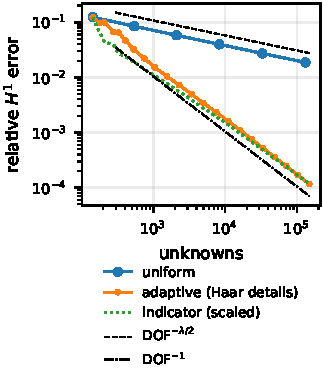
\includegraphics{trac_error.pdf}\\[-1pt]\small (a)\end{tabular} & \begin{tabular}{@{}c@{}}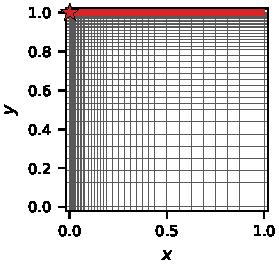
\includegraphics{trac_grid.pdf}\\[-1pt]\small (b)\end{tabular}\\
\end{tabular}\par\smallskip
\begin{tabular}{@{}c@{}}
\begin{tabular}{@{}c@{}}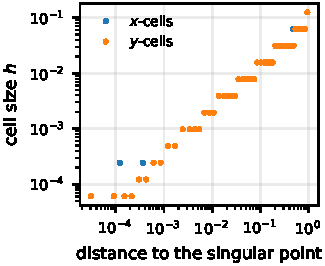
\includegraphics{trac_cellsize.pdf}\\[-1pt]\small (c)\end{tabular}\\
\end{tabular}\par\smallskip
\caption{Corner singularity at the end of a traction-free face ($\nu=0.3$). (a) Relative $H^1$ error versus number of unknowns for uniform and automatic refinement, with the scaled indicator. (b) Grid generated after 12 refinement cycles; the red edge is the traction-free face and the star marks the singular point. (c) Cell size versus distance to the singular point on the grid of (b).}\label{fig:trac}
\end{figure}

To put these numbers in context, we solved the same problem with biquadratic ($Q_2$) finite elements on
exactly the same grids, with the same type of solver: conjugate gradients preconditioned by fast
diagonalization (Table~\ref{tab:q2} and Fig.~\ref{fig:q2}). On a given grid, $Q_2$ is about 1.3 times more
accurate, but it has four times as many unknowns. In this benchmark, at equal accuracy, the collocation method needed about a quarter of the unknowns of $Q_2$. In our implementation and on our hardware this translated into about 3.6 times less end-to-end time
including assembly (about 1.1 times without it) and about 30\% less memory. These time and memory factors depend on implementation and
hardware; the factor in unknowns does not. A sparse direct solver was about 70 times slower than conjugate gradients with the
fast-diagonalization preconditioner (11.2~s at 193\,980 unknowns), so much of the speed-up often reported for structured methods comes from the
solver. We also preconditioned $Q_2$ with smoothed-aggregation algebraic multigrid (pyamg) using rigid-body near-nullspace modes. With the default pyamg settings, the number of CG iterations grew from 16 to 1700 as refinement stretched the cells, and CG did not converge within 2000 iterations from 193\,980 unknowns onwards; with an evolution strength measure designed for anisotropy, the number of CG iterations grew from 12 to 1589 as refinement stretched the cells, and CG did not converge within 2000 iterations from 283\,324 unknowns onwards. On the same grids, the fast-diagonalization preconditioner needed 11 to 20 CG iterations. These AMG settings were not tuned for the extreme anisotropy of adaptively refined tensor grids, and better-suited AMG variants may close the gap; the complete data are in \url{results/E13.json}.

\begin{table}[t]\centering\footnotesize
\caption{Collocation versus $Q_2$ finite elements on identical grids (every third refinement cycle).
Memory counts operators, factorizations and Krylov vectors.}\label{tab:q2}
\textit{(a) IHWC collocation: GMRES with the FDM preconditioner}\\[2pt]
\begin{tabular}{rr c ccc}
\toprule
cycle & unknowns & $e_{H^1}$ & setup (s) & solve (s) & MB\\
\midrule
0 & 144 & $1.23{\times}10^{-1}$ & 0.00 & 0.00 & 4.6\\
3 & 280 & $6.68{\times}10^{-2}$ & 0.00 & 0.00 & 4.7\\
6 & 532 & $3.22{\times}10^{-2}$ & 0.00 & 0.00 & 4.8\\
9 & 1550 & $1.05{\times}10^{-2}$ & 0.00 & 0.01 & 5.6\\
12 & 4982 & $3.42{\times}10^{-3}$ & 0.00 & 0.01 & 8.2\\
15 & 16182 & $1.11{\times}10^{-3}$ & 0.01 & 0.03 & 16.6\\
18 & 48960 & $3.59{\times}10^{-4}$ & 0.07 & 0.10 & 41.3\\
21 & 149008 & $1.17{\times}10^{-4}$ & 0.21 & 0.19 & 116.6\\
22 & 215644 & $8.03{\times}10^{-5}$ & 0.31 & 0.35 & 166.8\\
\bottomrule
\end{tabular}

\medskip
\textit{(b) $Q_2$ finite elements on the same grids, same cycles (rows) as in (a): CG with the FDM preconditioner, and sparse direct solve}\\[2pt]
\begin{tabular}{r c cccc}
\toprule
unknowns & $e_{H^1}$ & asm.\ (s) & CG (s) & MB & direct (s)\\
\midrule
480 & $7.22{\times}10^{-2}$ & 0.00 & 0.00 & 0.2 & 0.00\\
988 & $5.39{\times}10^{-2}$ & 0.01 & 0.00 & 0.3 & 0.00\\
1944 & $2.61{\times}10^{-2}$ & 0.01 & 0.00 & 0.7 & 0.01\\
5880 & $8.43{\times}10^{-3}$ & 0.01 & 0.01 & 2.0 & 0.04\\
19344 & $2.73{\times}10^{-3}$ & 0.04 & 0.03 & 6.8 & 0.26\\
63664 & $8.80{\times}10^{-4}$ & 0.13 & 0.07 & 22.7 & 1.76\\
193980 & $2.84{\times}10^{-4}$ & 0.44 & 0.17 & 69.4 & 11.18\\
592780 & $9.21{\times}10^{-5}$ & 1.45 & 0.57 & 212.6 & --\\
858676 & $6.33{\times}10^{-5}$ & 2.15 & 1.04 & 308.2 & --\\
\bottomrule
\end{tabular}
\end{table}
\begin{figure}[t]\centering
\begin{tabular}{@{}cc@{}}
\begin{tabular}{@{}c@{}}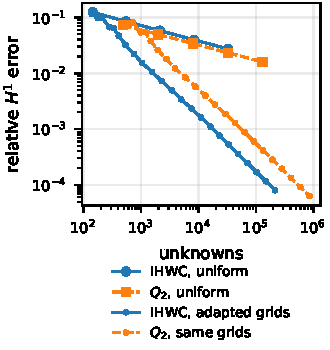
\includegraphics{q2_error.pdf}\\[-1pt]\small (a)\end{tabular} & \begin{tabular}{@{}c@{}}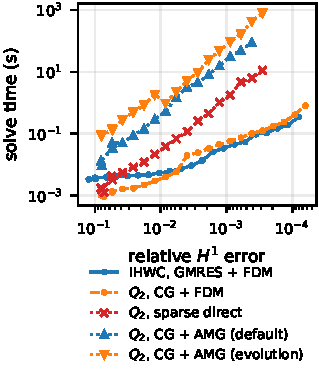
\includegraphics{q2_time.pdf}\\[-1pt]\small (b)\end{tabular}\\
\end{tabular}\par\smallskip
\caption{Collocation (IHWC) versus $Q_2$ finite elements on identical grids. (a) Error versus number of unknowns. (b) Solve time versus error for IHWC and for $Q_2$ with CG and the fast-diagonalization preconditioner, a sparse direct solver, and CG with algebraic multigrid (converged solves only).}\label{fig:q2}
\end{figure}

\subsection{Phase field: how many nodes does an interface need?}\label{sec:sharp}
Across an interface, $u$ goes from $-0.76$ to $0.76$ over a distance of $2\sqrt2\varepsilon$, so we measure
resolution in nodes per $\sqrt2\varepsilon$. For a planar interface solved exactly on discrete grids
(Fig.~\ref{fig:res}), plain HWCM is about twice as accurate as the standard three-point difference at every
resolution. The fourth-order operator pays off from about 1.5 nodes per $\sqrt2\varepsilon$. At 3.6 nodes it
is 25 times more accurate than finite differences, and at 7.2 nodes 110 times.

\begin{figure}[t]\centering
\begin{tabular}{@{}c@{}}
\begin{tabular}{@{}c@{}}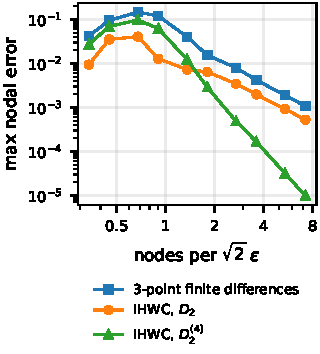
\includegraphics{resolution.pdf}\end{tabular}\\
\end{tabular}\par\smallskip
\caption{Planar interface ($\varepsilon=0.01$): maximum nodal error versus nodes per $\sqrt2\varepsilon$ (data in Table~S5).}\label{fig:res}
\end{figure}

For the Allen--Cahn six-fold star with $\varepsilon=0.004$, evolving under curvature flow, a $1024^2$
computation serves as the reference (Fig.~\ref{fig:star} and Table~\ref{tab:star}). On $256^2$, which gives
only 1.45 nodes per $\sqrt2\varepsilon$, the sharp tips move too slowly with $D_2$, while $D_2^{(4)}$ follows
the reference. $D_2^{(4)}$ on $256^2$ is as accurate in area as $D_2$ on $512^2$, with a quarter of the
unknowns, and on $512^2$ it is 16 times more accurate than $D_2$.

\begin{figure}[t]\centering
\begin{tabular}{@{}cc@{}}
\begin{tabular}{@{}c@{}}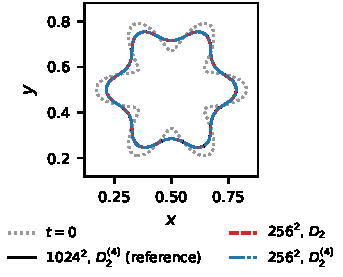
\includegraphics{star_levelsets.pdf}\\[-1pt]\small (a)\end{tabular} & \begin{tabular}{@{}c@{}}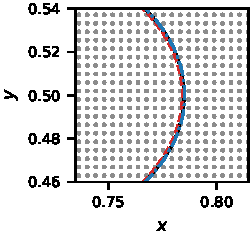
\includegraphics{star_zoom.pdf}\\[-1pt]\small (b)\end{tabular}\\
\end{tabular}\par\smallskip
\begin{tabular}{@{}c@{}}
\begin{tabular}{@{}c@{}}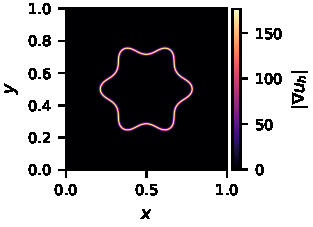
\includegraphics{star_gradient.pdf}\\[-1pt]\small (c)\end{tabular}\\
\end{tabular}\par\smallskip
\caption{Allen--Cahn star, $\varepsilon=0.004$, at $t=120$. (a) Zero level sets of the reference and of the $256^2$ solutions, and the initial interface. (b) Zoom at a tip, with the $256^2$ grid nodes. (c) Gradient magnitude of the reference solution.}\label{fig:star}
\end{figure}
\begin{table}[t]\centering\footnotesize
\caption{Allen--Cahn star ($\varepsilon=0.004$): maximum nodal error and area error against the $1024^2$
reference, and cost per step.}\label{tab:star}
\begin{tabular}{ll ccc}
\toprule
grid & operator & max nodal error & area error & ms per step\\
\midrule
$256^2$ & $D_2$ & $1.36{\times}10^{-1}$ & $2.43{\times}10^{-4}$ & 1.5\\
$256^2$ & $D_2^{(4)}$ & $5.27{\times}10^{-2}$ & $6.07{\times}10^{-5}$ & 1.5\\
$512^2$ & $D_2$ & $4.12{\times}10^{-2}$ & $6.88{\times}10^{-5}$ & 9.0\\
$512^2$ & $D_2^{(4)}$ & $2.63{\times}10^{-3}$ & $4.23{\times}10^{-6}$ & 9.2\\
$1024^2$ (reference) & $D_2^{(4)}$ & -- & -- & 93\\
\bottomrule
\end{tabular}
\end{table}

The most demanding case is Cahn--Hilliard with $\varepsilon=0.0015$ on $1024^2$, which gives 2.2 nodes per
$\sqrt2\varepsilon$; the whole interface spans about four nodes. With stabilized SAV ($S=4$), mass is
conserved to $10^{-17}$, both the modified and the physical energy decrease, $|u|$ stays below 1.03, and the
nodal profile across an interface coincides with the exact $\tanh$ profile. The largest computed gradient,
467, matches the exact value $1/(\sqrt2\varepsilon)=471$ (Fig.~\ref{fig:chsharp} and Table~\ref{tab:chsharp}).

\begin{figure}[t]\centering
\begin{tabular}{@{}ccc@{}}
\begin{tabular}{@{}c@{}}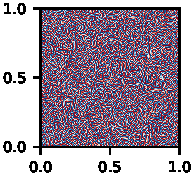
\includegraphics{ch_snap0.pdf}\\[-1pt]\small (a)\end{tabular} & \begin{tabular}{@{}c@{}}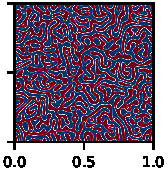
\includegraphics{ch_snap1.pdf}\\[-1pt]\small (b)\end{tabular} & \begin{tabular}{@{}c@{}}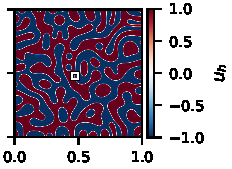
\includegraphics{ch_snap2.pdf}\\[-1pt]\small (c)\end{tabular}\\
\end{tabular}\par\smallskip
\begin{tabular}{@{}cc@{}}
\begin{tabular}{@{}c@{}}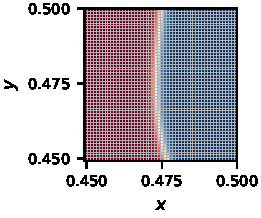
\includegraphics{ch_zoom.pdf}\\[-1pt]\small (d)\end{tabular} & \begin{tabular}{@{}c@{}}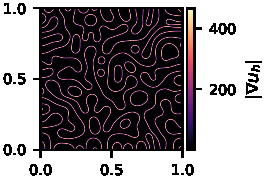
\includegraphics{ch_gradient.pdf}\\[-1pt]\small (e)\end{tabular}\\
\end{tabular}\par\smallskip
\begin{tabular}{@{}cc@{}}
\begin{tabular}{@{}c@{}}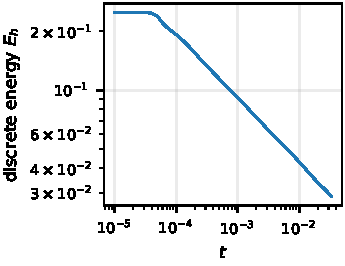
\includegraphics{ch_energy.pdf}\\[-1pt]\small (f)\end{tabular} & \begin{tabular}{@{}c@{}}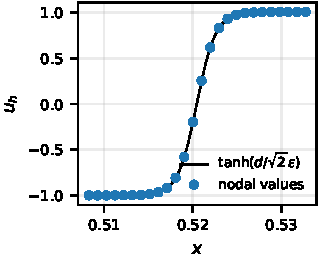
\includegraphics{ch_profile.pdf}\\[-1pt]\small (g)\end{tabular}\\
\end{tabular}\par\smallskip
\caption{Cahn--Hilliard with $\varepsilon=0.0015$ on $1024^2$. (a)--(c) Concentration at $t=0.0003$, $0.0033$ and $0.0333$; the box in (c) marks the region shown in (d). (d) Zoom in which each square is one node. (e) Gradient magnitude at the final time. (f) Discrete energy. (g) Nodal values along a grid line crossing an interface, compared with the $\tanh$ profile.}\label{fig:chsharp}
\end{figure}
\begin{table}[t]\centering\footnotesize
\caption{Cahn--Hilliard with $\varepsilon=0.0015$ on $1024^2$, stabilized SAV ($S=4$).}\label{tab:chsharp}
\begin{tabular}{p{0.52\textwidth}p{0.38\textwidth}}
\toprule
quantity & value\\
\midrule
grid and $\varepsilon$ & $1024^2$, 0.0015\\
nodes per $\sqrt2\varepsilon$ & 2.17\\
time steps & 1500$\times$$2{\times}10^{-7}$, 1500$\times$$2{\times}10^{-6}$, 1500$\times$$2{\times}10^{-5}$\\
largest mass deviation & $4.75{\times}10^{-18}$\\
largest step change of the modified energy & $-7.20{\times}10^{-8}$\\
largest change of $E_h$ between samples & $-3.37{\times}10^{-5}$\\
largest $|\nabla u_h|$ / planar-interface value $1/(\sqrt2\varepsilon)$ & 467 / 471\\
largest $|u_h|$ & 1.028\\
CPU time per step & 141 ms\\
\bottomrule
\end{tabular}
\end{table}
\begin{table}[t]\centering\footnotesize
\caption{Plain ($S=0$) versus stabilized ($S=4$) SAV for $\varepsilon=0.0015$: 150 steps from $t=0.0033$.}\label{tab:savstab}
\begin{tabular}{cc cccc}
\toprule
$S$ & $\Delta t$ & $\max|u_h|$ & $E_h$ (start $\to$ end) & $\xi$ & max $\Delta\tilde E$\\
\midrule
0 & $2{\times}10^{-5}$ & 77.33 & 0.062 $\to$ 503.681 & -0.00003 & $-4.59{\times}10^{-5}$\\
0 & $5{\times}10^{-6}$ & 122.58 & 0.062 $\to$ 801.433 & -0.00002 & $-3.23{\times}10^{-5}$\\
4 & $2{\times}10^{-5}$ & 1.04 & 0.062 $\to$ 0.050 & 1.00002 & $-5.02{\times}10^{-5}$\\
4 & $5{\times}10^{-6}$ & 1.04 & 0.062 $\to$ 0.058 & 1.00000 & $-2.27{\times}10^{-5}$\\
\bottomrule
\end{tabular}
\end{table}

\subsection{When not to use the method}\label{sec:compare}
Because every uniform-grid operator considered here is diagonalized by the same cosine transform, we
could compare five of them within the identical solver: the three-point difference, $D_2$, $D_2^{(4)}$,
the classical compact (Pad\'e) scheme, and the cosine pseudo-spectral method (Fig.~\ref{fig:compare} and
Table~S14). Plain HWCM beats the three-point difference by a factor of two, and the compact scheme is about
1.4 times more accurate than $D_2^{(4)}$. For smooth problems on uniform boxes with zero-flux or periodic
conditions, however, the pseudo-spectral method is far more accurate than all others. For such problems we
recommend pseudo-spectral methods. The strength of the present method lies in graded and adaptive grids,
prescribed values and tractions, and singular solutions. The elastostatic formulation is also not robust
as Poisson's ratio approaches one half (Tables~S1 and~S2).

\begin{figure}[t]\centering
\begin{tabular}{@{}c@{}}
\begin{tabular}{@{}c@{}}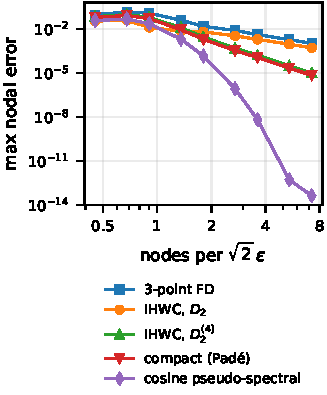
\includegraphics{scheme_comparison.pdf}\end{tabular}\\
\end{tabular}\par\smallskip
\caption{Planar interface: maximum nodal error versus resolution for five operators.}\label{fig:compare}
\end{figure}

\subsection{Performance}
A phase-field time step costs $O(N^d\log N)$ operations with fast cosine transforms. On the CPU of Table~\ref{tab:env} this amounted to between $10^{7}$ and $5\times10^{7}$ unknowns per second (Table~\ref{tab:perf}). Absolute timings
depend on the hardware; the complexity does not. GPU timings were measured on an NVIDIA GeForce RTX 3050 Ti Laptop GPU (CUDA 13.2, CuPy 14.2.0); times are per step after warm-up, with device synchronization.

\begin{table}[t]\centering\footnotesize
\caption{Time per Cahn--Hilliard time step with $D_2^{(4)}$.}\label{tab:perf}
\textit{(a) CPU, double precision (ms per step)}\\[2pt]
\begin{tabular}{rr r cc}
\toprule
$d$ & $N$ & unknowns & GEMM & DCT\\
\midrule
2 & 128 & 16384 & 0.77 & 0.34\\
2 & 256 & 65536 & 2.25 & 1.55\\
2 & 512 & 262144 & 12.69 & 12.02\\
2 & 1024 & 1048576 & 146.23 & 103.26\\
2 & 2048 & 4194304 & -- & 363.06\\
3 & 32 & 32768 & 0.99 & 1.06\\
3 & 64 & 262144 & 8.11 & 9.41\\
3 & 128 & 2097152 & 191.31 & 189.90\\
\bottomrule
\end{tabular}

\medskip
\textit{(b) GPU (ms per step)}\\[2pt]
\begin{tabular}{rr cc cc}
\toprule
& & \multicolumn{2}{c}{double precision} & \multicolumn{2}{c}{single precision}\\
$d$ & $N$ & GEMM & DCT & GEMM & DCT\\
\midrule
2 & 128 & 1.10 & 2.13 & 1.18 & 2.17\\
2 & 256 & 3.14 & 2.59 & 3.29 & 2.18\\
2 & 512 & 13.98 & 2.89 & 11.21 & 2.88\\
2 & 1024 & 75.91 & 10.63 & 76.42 & 10.62\\
2 & 2048 & 589.88 & 44.33 & 591.10 & 44.18\\
3 & 32 & 1.46 & 2.93 & 1.80 & 2.94\\
3 & 64 & 3.35 & 3.66 & 3.42 & 3.63\\
3 & 128 & 35.14 & 31.91 & 34.97 & 32.05\\
\bottomrule
\end{tabular}
\end{table}

%==========================================================================
\section{Practical guidelines}\label{sec:guide}
%==========================================================================
Table~\ref{tab:guide} summarizes the choices that worked in our computations.

\begin{table}[t]\centering\footnotesize
\caption{Practical recommendations.}\label{tab:guide}
\begin{tabular}{p{0.22\textwidth}p{0.72\textwidth}}
\toprule
Decision & Recommendation\\
\midrule
Plain or corrected operator & Use $D_2^{(4)}$ for zero-flux or periodic problems, since it costs nothing extra. With general prescribed values, use $D_2$, because the correction does not raise the order there.\\
When not to use IHWC & For smooth or phase-field problems on uniform boxes with zero-flux or periodic conditions, a cosine pseudo-spectral operator is far more accurate at the same cost (Section~\ref{sec:compare}).\\
Interface resolution & Use at least 1.5 nodes per $\sqrt2\varepsilon$ with $D_2^{(4)}$. Expect a nodal error of about $10^{-3}$ at 2 to 3 nodes, and about $10^{-4}$ at 3.5 nodes (Table~S5).\\
Time stepping (AC, CH) & Use SAV-BDF2 with the smallest stabilization that keeps $\xi=r/\sqrt{E_{1,h}+C}$ near one: $S\approx1$ to 2 for $\Delta t\lesssim\varepsilon^2$, and 2 to 4 for larger steps (Table~S17). Keep $\Delta t$ of order $\varepsilon^2$ when the coarsening dynamics matter, and verify by halving $\Delta t$; $\xi\approx1$ alone does not guarantee accuracy.\\
Solver & On uniform grids, use cosine or sine transforms. On graded grids, use fast diagonalization (well defined by Theorem~\ref{thm:spectrum}) with the backward-error check and Bartels--Stewart fallback, and heed the sensitivity flag based on $\kappa_{\mathrm{Syl}}$. For coupled systems such as elasticity, use GMRES with the block preconditioner.\\
Adaptivity at singularities & Use the Haar-detail indicator with D\"orfler parameter $\theta\approx0.6$, a neighbour ratio of at most two, and an initial grid of $8\times8$ cells.\\
Traction conditions & Collocate tractions plainly at edge midpoints, without enhancement, and use the two normal-stress conditions at traction--traction corners.\\
Near incompressibility & Avoid $\nu>0.45$ with the present formulation (Tables~S1 and~S2).\\
\bottomrule
\end{tabular}
\end{table}

%==========================================================================
\section{Limitations}\label{sec:limits}
%==========================================================================
The fast solvers require rectangular domains; the full L-shaped domain and curved boundaries need
multi-patch coupling or geometry maps. Refinement is anisotropic but not local, which costs a constant
factor of about four in cells at point singularities. Proved results and observations should be
distinguished. Proved are the three-term identity, the real spectrum on every grid, the fourth-order
correction and the symmetric structure on uniform grids, exact mass conservation, and the decay of the
modified energy on uniform grids. Observed, but not proved, are the conditioning of the eigenvectors, the
decay of the physical energy, the boundedness of $u$, the reliability of the refinement indicator, the
optimal adaptive rates, and the mesh-independent iteration counts. The last of these hold for compressible
materials only. Comparisons with adaptive isogeometric collocation and with multigrid-preconditioned finite
elements are still missing.

%==========================================================================
\section{Conclusions}
%==========================================================================
Rewritten in nodal form, Haar wavelet collocation is midpoint quadratic-spline collocation, and its
second-derivative operator has real, simple and nonpositive eigenvalues on every strictly increasing grid
(Theorem~\ref{thm:spectrum}). Fast diagonalization is therefore well defined on any graded or adaptively
refined tensor grid. In floating-point arithmetic it was backward stable on random and adversarial grids,
and an inexpensive backward-error check with a Bartels--Stewart fallback guards against failures it can
detect; forward accuracy remains limited by the conditioning of the discrete problem, which the code
estimates and flags. The structure replaces the dense HWCM systems by fast tensor solves, gives a
fourth-order correction at no cost on uniform grids with zero-flux conditions, and supports
mass-conserving phase-field schemes with a modified energy law that, with stabilization, resolved
interfaces with about four nodes across the transition layer. For compressible elastostatics with
tractions, refinement driven by Haar detail coefficients recovered the optimal convergence rate at the
tested corner singularities, and in a benchmark against biquadratic finite elements on identical grids the
method needed about a quarter of the unknowns. For smooth problems on uniform boxes, pseudo-spectral
methods remain the better choice.


\section*{Declarations}
\paragraph{Funding} No funding was received for conducting this study.

\paragraph{Competing interests} The author has no relevant financial or non-financial interests to disclose.

\paragraph{Author contributions} Farshid Mossaiby: Conceptualization, Methodology, Software, Validation,
Formal analysis, Investigation, Resources, Data curation, Writing -- original draft, Writing -- review and
editing, Visualization, Supervision, Project administration.

\paragraph{Code availability} The implementation, the tests and the scripts that produce every table and
figure are openly available at \repo; the version used in this paper is the GitHub release v1.1. Dependencies
are listed in \texttt{requirements.txt} (CPU) and \texttt{requirements-gpu.txt} (GPU).

\paragraph{Data availability} All data in this paper are generated by the scripts in the repository; the
stored results (\texttt{results/*.json}) and the generated tables are part of release v1.1.


\appendix
%==========================================================================
\section{Proofs of Theorem~\ref{thm:identity}, Corollary~\ref{cor:ops} and Theorem~\ref{thm:spectrum}}\label{app:proofs}
%==========================================================================
\begin{proof}[of Theorem~\ref{thm:identity}]
Let $\sigma_k=s'(t_k)$. On $I_k$, $s'(x)=\sigma_k+c_k(x-t_k)=\sigma_{k-1}+c_k(x-t_{k-1})$, hence
$\sigma_k-\sigma_{k-1}=c_kh_k$. Integrating $s'$ from $m_k$ to $m_{k+1}$ across $t_k$ gives
\begin{align*}
U_{k+1}-U_k&=\int_{m_k}^{t_k}\!\big(\sigma_k+c_k(x-t_k)\big)dx+\int_{t_k}^{m_{k+1}}\!\big(\sigma_k+c_{k+1}(x-t_k)\big)dx\\
&=\sigma_kd_k-\frac{c_kh_k^2}{8}+\frac{c_{k+1}h_{k+1}^2}{8}.
\end{align*}
Dividing by $d_k$, subtracting the same relation for $k-1$, and using $\sigma_k-\sigma_{k-1}=c_kh_k$
gives~\eqref{eq:interior}. At the left end, $U_1-g_0=\sigma_0h_1/2+c_1h_1^2/8$, so
$2(U_1-g_0)/h_1=\sigma_0+c_1h_1/4$; subtracting this from the relation for $(U_2-U_1)/d_1$
gives~\eqref{eq:dirrow}. If $\sigma_0=0$, then $\sigma_1=c_1h_1$ and~\eqref{eq:neurow} follows. The right
end is analogous. The expressions for $s'(m_k)$ and for the end slopes used in Algorithm~1 follow from
$s'=\sigma_0+\int s''$. \qed
\end{proof}

\begin{proof}[of Corollary~\ref{cor:ops}]
The off-diagonal entries of column $k$ of $A$ are positive and sum to $h_k^2/(8d_{k-1})+h_k^2/(8d_k)$, so
the column-dominance margin is $h_k-h_k^2/(4d_{k-1})-h_k^2/(4d_k)>0$, because $d_j>h_k/2$. For an end column
with a prescribed value the margin is $3h_1/4-h_1^2/(4d_1)>h_1/4$, and for a zero-slope end column it is
$h_1-h_1^2/(4d_1)>h_1/2$. Summing the entries of column $k$ in~\eqref{eq:interior} and~\eqref{eq:neurow}, the
terms $h_k^2/(8d_j)$ cancel and the sum is $h_k$; for a prescribed-value end column it is $3h_1/4$. The
collocation problem reads $LU=Af-b$. The matrix $-L$ is symmetric, irreducible and weakly diagonally
dominant, with zero row sums in the interior rows. A prescribed value adds $2/h_1$ (or $2/h_N$) to the
corresponding diagonal entry, which makes $-L$ irreducibly diagonally dominant and hence nonsingular. If
the slope vanishes at both ends, all row sums of $L$ are zero, so its kernel is spanned by the constant
vector, and, since $L$ is symmetric, $LU=Af$ is solvable if and only if $\mathbf 1^{\mathsf T}Af=0$. Because
$\mathbf 1^{\mathsf T}A=h^{\mathsf T}$, this is the condition $\sum_kh_kf(m_k)=0$. \qed
\end{proof}

\begin{proof}[of Theorem~\ref{thm:spectrum}]
We use three standard facts~\cite{gantmacher2002oscillation,fallat2011totally}. (F1) A tridiagonal matrix
with nonnegative entries is totally nonnegative (all minors nonnegative) if and only if all its principal
minors are nonnegative. (F2) If $B$ is nonsingular and totally nonnegative, then $JB^{-1}J$ is totally
nonnegative, where $J=\mathrm{diag}((-1)^i)$; products of totally nonnegative matrices are totally
nonnegative (Cauchy--Binet). (F3) A totally nonnegative matrix is oscillatory if it is nonsingular and its
entries next to the diagonal are positive; the eigenvalues of an oscillatory matrix are real, positive and
simple (Gantmacher--Krein).

First let a value be prescribed at one or both ends. Then $-L$ is an irreducible tridiagonal matrix with
positive diagonal, negative off-diagonal entries, zero row sums in the interior and a positive row sum in at
least one end row. It is therefore a nonsingular M-matrix, and all its principal minors are positive. The
matrix $J(-L)J$ has the same principal minors and nonnegative entries, so it is totally nonnegative by (F1).
By (F2), $(-L)^{-1}=J\,(J(-L)J)^{-1}J$ is totally nonnegative; it is also entrywise positive, as the inverse
of an irreducible M-matrix. The matrix $A$ has nonnegative entries, and $JAJ$ is a Z-matrix that is strictly
diagonally dominant by columns (Corollary~\ref{cor:ops}), hence an M-matrix. Its principal minors, which are
those of $A$, are therefore positive, and $A$ is totally nonnegative by (F1). The product $P=(-L)^{-1}A$ is
totally nonnegative and nonsingular, and it is entrywise positive, since $(-L)^{-1}$ is entrywise positive
and $A$ is nonnegative with a positive diagonal. By (F3), $P$ is oscillatory and has $N$ real, positive,
simple eigenvalues. Since $D_2=A^{-1}L=-P^{-1}$, the eigenvalues of $D_2$ are real, negative and simple.

If the slope vanishes at both ends, $L$ is singular. Let $0<\sigma<8/\max_kh_k^2$, and consider
$-(L-\sigma A)=-L+\sigma A$. Its off-diagonal entries are $-1/d_k+\sigma h_j^2/(8d_k)<0$, and its columns have
the positive dominance margin $\sigma h_k$, because the columns of $L$ sum to zero and those of $A$ sum to
$h_k$ (Corollary~\ref{cor:ops}). It is therefore a nonsingular M-matrix, and the argument above applies to
$(-L+\sigma A)^{-1}A$. Hence $A^{-1}L-\sigma I$ has real, negative, simple eigenvalues, so the eigenvalues of
$D_2$ are real, simple and smaller than $\sigma$. Since $\sigma$ can be arbitrarily small, they are
nonpositive, and the constant vector spans the kernel. Real simple eigenvalues of a real matrix have real
eigenvectors, so $V$ is real. Corollary~\ref{cor:tensor} follows because the tensor-product operator is a
sum of commuting Kronecker factors, each diagonalized by its $V_m$. \qed
\end{proof}

\begin{thebibliography}{99}
\bibitem{chen1997haar} C.F. Chen, C.H. Hsiao, Haar wavelet method for solving lumped and distributed-parameter systems, IEE Proc. Control Theory Appl. 144 (1997) 87--94.
\bibitem{lepik2005numerical} \"U. Lepik, Numerical solution of differential equations using Haar wavelets, Math. Comput. Simul. 68 (2005) 127--143.
\bibitem{lepik2011solving} \"U. Lepik, Solving PDEs with the aid of two-dimensional Haar wavelets, Comput. Math. Appl. 61 (2011) 1873--1879.
\bibitem{lepik2014book} \"U. Lepik, H. Hein, Haar Wavelets: With Applications, Springer, Cham, 2014.
\bibitem{majak2015accuracy} J. Majak, B. Shvartsman, K. Karjust, M. Mikola, A. Haavaj\~oe, M. Pohlak, On the accuracy of the Haar wavelet discretization method, Compos. B Eng. 80 (2015) 321--327.
\bibitem{majak2015convergence} J. Majak, B.S. Shvartsman, M. Kirs, M. Pohlak, H. Herranen, Convergence theorem for the Haar wavelet based discretization method, Compos. Struct. 126 (2015) 227--232.
\bibitem{majak2018higher} J. Majak, M. Pohlak, K. Karjust, M. Eerme, J. Kurnitski, B.S. Shvartsman, New higher order Haar wavelet method: Application to FGM structures, Compos. Struct. 201 (2018) 72--78.
\bibitem{ratas2021solving} M. Ratas, J. Majak, A. Salupere, Solving nonlinear boundary value problems using the higher order Haar wavelet method, Mathematics 9 (2021) 2809.
\bibitem{dubeau2004nonuniform} F. Dubeau, S. Elmejdani, R. Ksantini, Non-uniform Haar wavelets, Appl. Math. Comput. 159 (2004) 675--693.
\bibitem{lepik2008nonuniform} \"U. Lepik, Solving integral and differential equations by the aid of non-uniform Haar wavelets, Appl. Math. Comput. 198 (2008) 326--332.
\bibitem{oruc2019nonuniform} \"O. Oru\c{c}, A non-uniform Haar wavelet method for numerically solving two-dimensional convection-dominated equations and two-dimensional near singular elliptic equations, Comput. Math. Appl. 77 (2019) 1799--1820.
\bibitem{houstis1988quadratic} E.N. Houstis, C.C. Christara, J.R. Rice, Quadratic-spline collocation methods for two-point boundary value problems, Int. J. Numer. Methods Eng. 26 (1988) 935--952.
\bibitem{christara1994quadratic} C.C. Christara, Quadratic spline collocation methods for elliptic partial differential equations, BIT 34 (1994) 33--61.
\bibitem{christara2006optimal} C.C. Christara, K.S. Ng, Optimal quadratic and cubic spline collocation on nonuniform partitions, Computing 76 (2006) 227--257.
\bibitem{christara2006adaptive} C.C. Christara, K.S. Ng, Adaptive techniques for spline collocation, Computing 76 (2006) 259--277.
\bibitem{christara2002fast} C.C. Christara, K.S. Ng, Fast Fourier transform solvers and preconditioners for quadratic spline collocation, BIT 42 (2002) 702--739.
\bibitem{auricchio2010isogeometric} F. Auricchio, L. Beir\~ao da Veiga, T.J.R. Hughes, A. Reali, G. Sangalli, Isogeometric collocation methods, Math. Models Methods Appl. Sci. 20 (2010) 2075--2107.
\bibitem{schillinger2013isogeometric} D. Schillinger, J.A. Evans, A. Reali, M.A. Scott, T.J.R. Hughes, Isogeometric collocation: Cost comparison with Galerkin methods and extension to adaptive hierarchical NURBS discretizations, Comput. Methods Appl. Mech. Engrg. 267 (2013) 170--232.
\bibitem{delorenzis2015isogeometric} L. De Lorenzis, J.A. Evans, T.J.R. Hughes, A. Reali, Isogeometric collocation: Neumann boundary conditions and contact, Comput. Methods Appl. Mech. Engrg. 284 (2015) 21--54.
\bibitem{lynch1964direct} R.E. Lynch, J.R. Rice, D.H. Thomas, Direct solution of partial difference equations by tensor product methods, Numer. Math. 6 (1964) 185--199.
\bibitem{bartels1972solution} R.H. Bartels, G.W. Stewart, Solution of the matrix equation $AX+XB=C$, Commun. ACM 15 (1972) 820--826.
\bibitem{sangalli2016isogeometric} G. Sangalli, M. Tani, Isogeometric preconditioners based on fast solvers for the Sylvester equation, SIAM J. Sci. Comput. 38 (2016) A3644--A3671.
\bibitem{shen2018scalar} J. Shen, J. Xu, J. Yang, The scalar auxiliary variable (SAV) approach for gradient flows, J. Comput. Phys. 353 (2018) 407--416.
\bibitem{gantmacher2002oscillation} F.R. Gantmacher, M.G. Krein, Oscillation Matrices and Kernels and Small Vibrations of Mechanical Systems, revised ed., AMS Chelsea Publishing, Providence, RI, 2002.
\bibitem{dorfler1996convergent} W. D\"orfler, A convergent adaptive algorithm for Poisson's equation, SIAM J. Numer. Anal. 33 (1996) 1106--1124.
\bibitem{williams1952stress} M.L. Williams, Stress singularities resulting from various boundary conditions in angular corners of plates in extension, J. Appl. Mech. 19 (1952) 526--528.
\bibitem{dyksen1987tensor} W.R. Dyksen, Tensor product generalized ADI methods for separable elliptic problems, SIAM J. Numer. Anal. 24 (1987) 59--76.
\bibitem{sun1999spectral} W. Sun, Spectral analysis of Hermite cubic spline collocation systems, SIAM J. Numer. Anal. 36 (1999) 1962--1975.
\bibitem{bialecki1995matrix} B. Bialecki, G. Fairweather, Matrix decomposition algorithms in orthogonal spline collocation for separable elliptic boundary value problems, SIAM J. Sci. Comput. 16 (1995) 330--347.
\bibitem{bialecki2011matrix} B. Bialecki, G. Fairweather, A. Karageorghis, Matrix decomposition algorithms for elliptic boundary value problems: a survey, Numer. Algorithms 56 (2011) 253--295.
\bibitem{fallat2011totally} S.M. Fallat, C.R. Johnson, Totally Nonnegative Matrices, Princeton University Press, Princeton, NJ, 2011.
\end{thebibliography}

\end{document}
